\documentclass[10pt,a4paper]{article}

\usepackage[utf8]{inputenc}
\usepackage[italian]{babel}
\usepackage{amsmath}
\usepackage{amsfonts}
\usepackage{amssymb}
\usepackage{graphicx}

\usepackage[left=2cm,right=2cm,top=2cm,bottom=2cm]{geometry}
\geometry{a4paper}

\usepackage{booktabs} % for much better looking tables
\usepackage{verbatim}
\usepackage{subfig} % make it possible to include more than one captioned figure/table in a single 

\usepackage{fancyhdr} % This should be set AFTER setting up the page geometry
\pagestyle{fancy} % options: empty , plain , fancy
\renewcommand{\headrulewidth}{0pt} % customise the layout...
\lhead{}\chead{}\rhead{}
\lfoot{}\cfoot{\thepage}\rfoot{}

%%% SECTION TITLE APPEARANCE
\usepackage{sectsty}
%\allsectionsfont{\sffamily\mdseries\upshape} % (See the fntguide.pdf for font help)
% (This matches ConTeXt defaults)

\title{Esercitazione 1: Misure di tensione, corrente, tempi, frequenze}
\author{Gruppo bE \\ Alessandro Candido, Roberto Ribatti}
\date{\today} 

\begin{document}
\maketitle

\section{Scopo e strumentazione}
Lo scopo dell'esercitazione è di impratichirsi con la strumentazione disponibile in laboratorio. Abbiamo usato multimetro, oscilloscopio, alimentatore da banco e generatore di funzioni d'onda.

\section{Misure di tensione e corrente}

\subsection{Partitore di tensione $\sim1\text{k}\Omega$}
Si è costruito il partitore di tensione illustrato nella scheda (Figura 1) usando due resistenze $R_1 = 976 \pm 9~\Omega$ e $R_2 = 974 \pm 9 ~\Omega$.
Si è variata la tensione dell'alimentatore tra $0~V$ e $10~V$ e volta per volta si è misurata con il multimetro digitale la tensione erogata dall'alimentatore $V_{in}$ e ai capi della resistenza $R2$, $V_{out}$. Gli errori sono stati ottenuti usando le indicazioni del manuale del multimetro.
Il rapporto atteso tra le due tensioni è $1/(1+(R_1/R_2))=0.499 \pm 0.005$. 
I risultati della misura sono qui di seguito riportati:

\begin{figure}[h]
\centering
\begin{minipage}[b]{.6\textwidth}
	\centering
	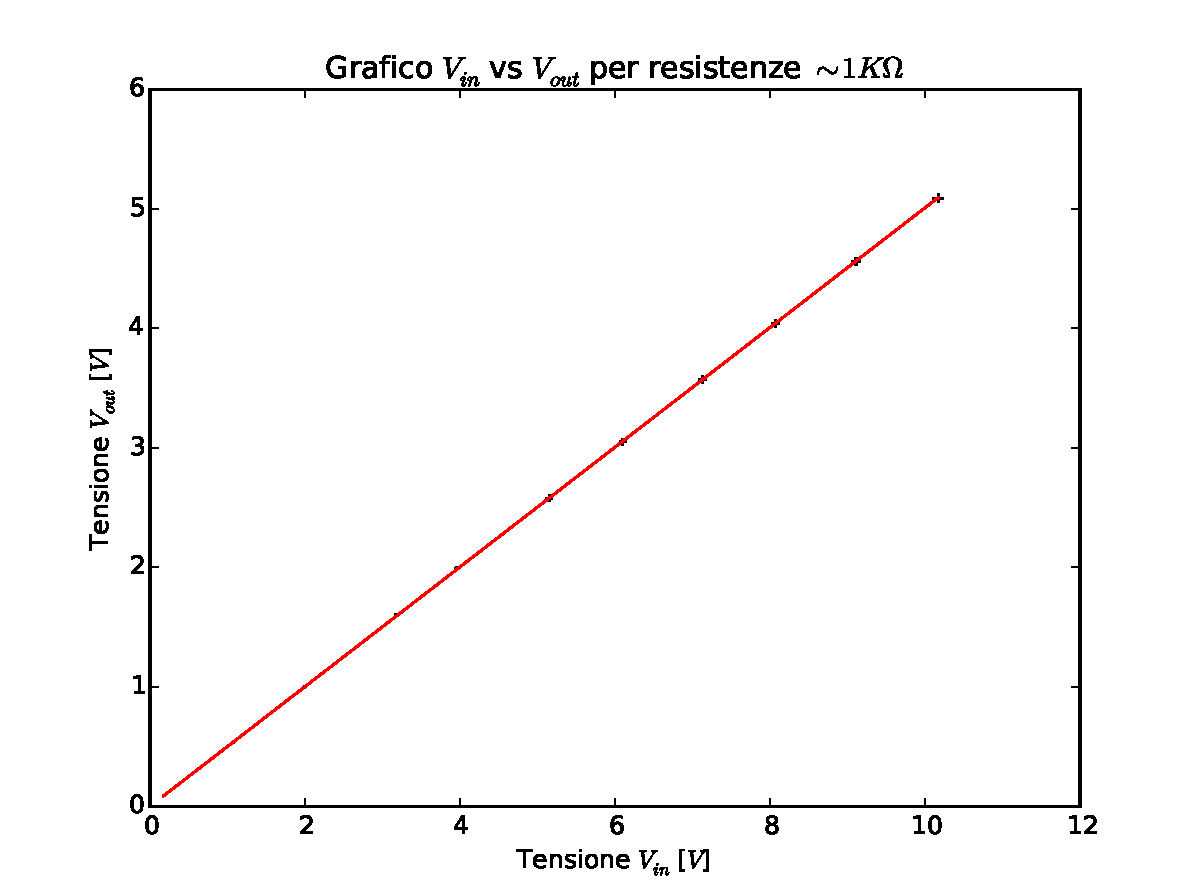
\includegraphics[scale=.5\textwidthwidth]{../grafici/fit_1KOhm.pdf}
	\caption{Partitore di tensione.}
	\label{f:par1}
\end{minipage}\hfill
\begin{minipage}[b]{.35\textwidth}
	\centering
	\input{../tabelle/tab_1KOhm.txt}
	\captionof{table}{Didascalia della tabella}\label{...}
\end{minipage}\hspace*{\fill}
\end{figure}


Come atteso il rapporto tra le tensioni è costante, ovvero la relazione che lega $V_{out}$ e $V_{in}$ è lineare.
Abbiamo eseguito un fit lineare numerico che tenesse conto degli errori su entrambi gli assi poiché gli errori sono confrontabili. I risultati del fit sono: $V_{out}/V_{in}=0.5009 \pm 0.0016$, e un valore pari a $(0.2\pm 0.8) mV$ del'intercetta. Abbiamo ottenuto  $\chi^2/\text{ndof}= 1.16/9$.

Il valore del $\chi^2$ è lontano dal valor medio della distribuzione, probabilmente perché le incertezze del tester digitale sono sovrastimate. La misura tuttavia è da confrontare con quella prevista a partire dalla misura delle resistenze, e risulta compatibile entro gli errori. Inoltre per l'intercetta si ha una misura di $0$.

\subsection{Partitore di tensione $\sim4\text{M}\Omega$}
Si sono usate adesso resistenze $R_3=4.87 \pm 7 ~M\Omega$ e $R_4=3.70 \pm 6 ~M\Omega$ e si è proceduto alla stessa misura del punto precedente. In questo caso la relazione è lineare, ma non col coefficiente atteso se l'impedenza di ingresso del multimetro fosse trascurabile. Questa infatti da manuale ammonta a $10 ~ \text{M}\Omega$ , ed è confrontabile con le resistenze in gioco.

\begin{figure}[h]
\centering
\begin{minipage}[b]{.6\textwidth}
	\centering
	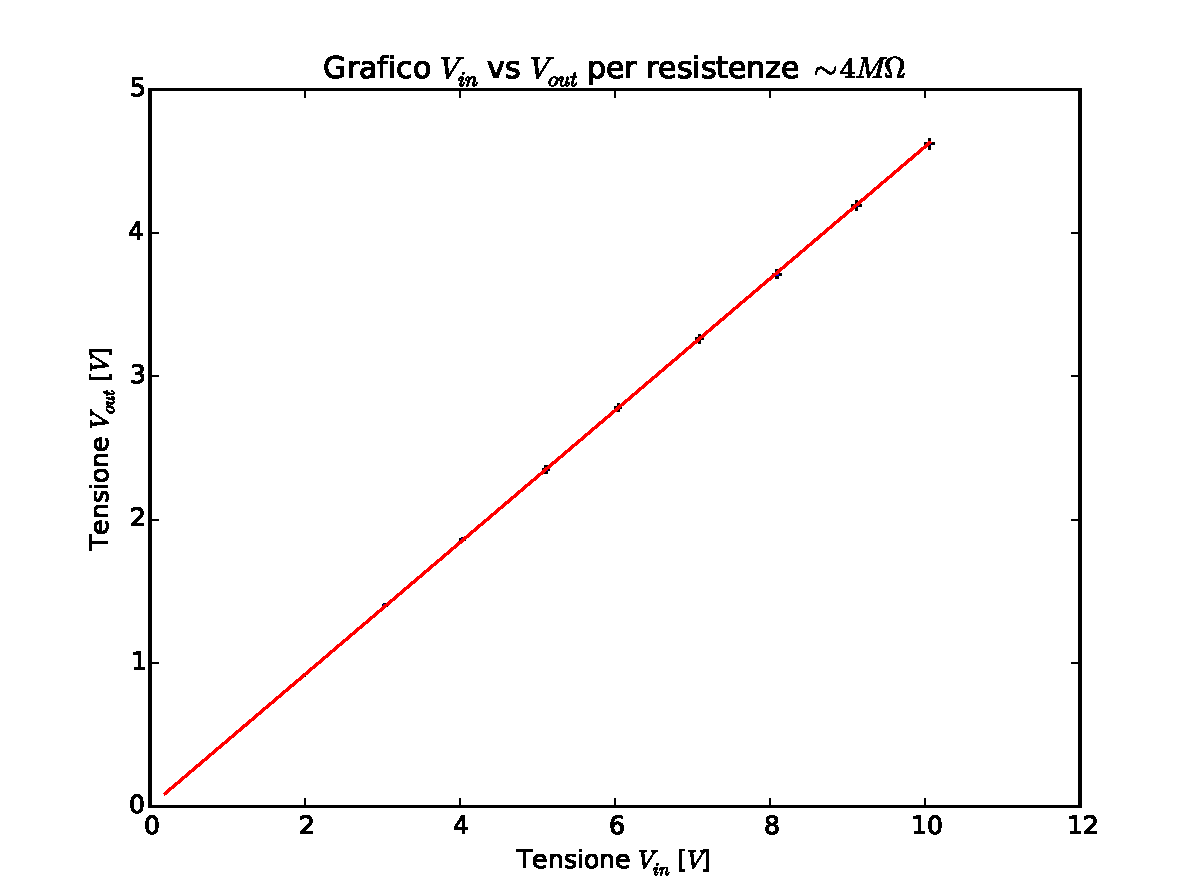
\includegraphics[scale=.5\textwidthwidth]{../grafici/fit_4MOhm.pdf}
	\caption{Partitore di tensione.}
	\label{f:par2}
\end{minipage}\hfill
\begin{minipage}[b]{.35\textwidth}
	\centering
	\input{../tabelle/tab_4MOhm.txt}
	\captionof{table}{Didascalia della tabella}\label{...}
\end{minipage}\hspace*{\fill}
\end{figure}

Il fit è stato eseguito come al punto precedente e i valori ottenuti sono $V_{out}/V_{in} = 0.4600 \pm 0.0015$ e per l'intercetta $0.2 \pm 0.8 mV$. Si è ottenuto inoltre $\chi^2 / \text{ndof} = 1.94 / 9$.

Perciò sia per quanto riguarda l'intercetta che il $\chi^2$ si applicano le stesse considerazioni del punto precedente. Per quanto riguarda la pendenza della retta ci saremmo attesi un valore pari a  $1/(1+(R_1/R_2))=0.568 \pm 0.004$, che evidentemente non è compatibile con quanto risulta dal fit. Il motivo di ciò è, come detto sopra, l'impedenza d'ingresso del tester digitale.

Considerando l'impedenza del tester si ottiene per la pendenza $\frac{1}{1 + R_1 (1/R_2 + 1/R_T)}$, dove si è indicato con $R_T$ la resistenza interna del tester. Invertendo la formula si trova $R_T = 11.6 \pm 0.8 \text{M}\Omega$.

\subsection{Partitore di corrente}


\section{Uso dell'oscilloscopio}

\section{Misure di frequenza e tempo}

\section{Trigger dell'oscilloscopio}
Si è osservato il segnale di pulse del generatore di forme d'onda, confrontandolo sia con un'onda quadra che con una sinusoide, entrambe prodotte dallo stesso generatore.
La relazione fra il segnale di sincronizzazione e la portante dell'onda osservata è uno sfasamento di mezzo periodo, come appare evidente nel caso dell'onda quadra, e si verifica anche per la sinusoide identificando lo stato alto del pulse con il fronte di salita della sinusoide e il basso con la discesa.

I segnali osservati sono riportati in \figurename{\ref{f:pulse}}.
	
\begin{figure}[h]
	\centering
	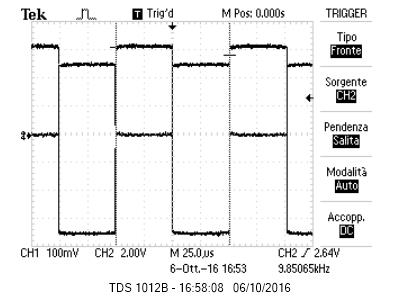
\includegraphics[scale=0.6]{../Oscilloscopio/trig_pulse_square.jpg}
	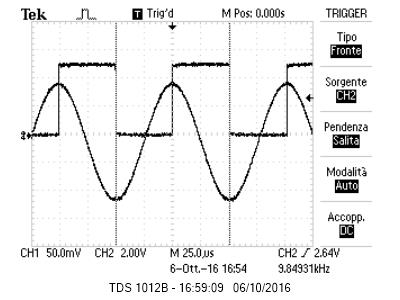
\includegraphics[scale=0.6]{../Oscilloscopio/trig_pulse_sin.jpg}
	\caption{Segnale di pulse a confronto con un'onda quadra e una sinusoide}
	\label{f:pulse}
\end{figure}

Si è dunque eseguita l'ultima parte dell'esercitazione, visualizzando un'onda quadra prodotta dal generatore a una frequenza di $\sim880~\text{kHz}$.
Così come si osserva dalla \figurename{\ref{sqmhz}} è evidente che il tempo impiegato dai fronti di salita e discesa è non nullo, anche se al genratore è stata richiesta un'onda quadra. I valori misurati sono $t_{raise} = (64.0 \pm )~\text{n}s$ e $t_{fall} = (64.0 \pm )~\text{n}s$, cioè uguali entro l'errore. %c'è da stimare gli errori sulla misura dei tempi, e forse anche quello sulla frequenza
Per quanto riguarda invece i fenomeni di overshoot, undershoot essi si possono osservare qualitativamente dalla \figurename{\ref{sqmhz}}, ma alla frequenza scelta non sono ancora troppo marcati (rimangono piccoli rispetto all'ampiezza dell'onda quadra).
%ci siamo scordati il duty cicle attivo, e dunque non era al 50%; quindi o lo nascondiamo sotto il tappeto, magari addirittura tagliando l'immagine, oppure lo dichiariamo

\begin{figure}[h]
	\centering
	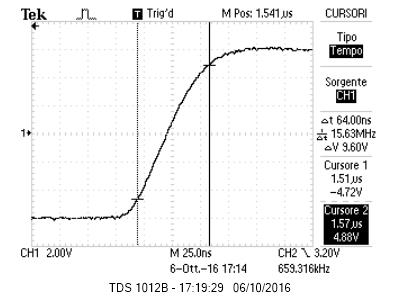
\includegraphics[scale=0.6]{../Oscilloscopio/raise_time.jpg}
	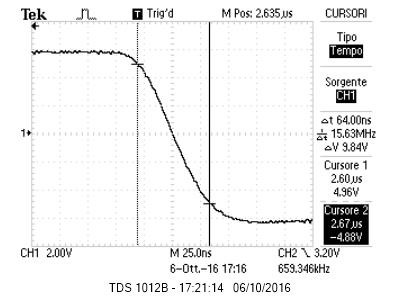
\includegraphics[scale=0.6]{../Oscilloscopio/fall_time.jpg}
	\caption{Fronti di salita e di discesa dell'onda quadra}
	\label{f:sqmhz}
\end{figure}

\section{Conclusioni e commenti finali}

\end{document}
